% mainfile: ../../../../master.tex
\subsection{Migration of nucleic acids in agarose gel}
% The part of the label after the colon must match the file name. Otherwise,
% conditional compilation based on task labels does NOT work.
\label{task:20180210_cj1}
\tags{lab,pcr,emp}
\authors{cj}
%\files{}
%\persons{} % Here, you can write the persons who attented the meeting

I basically repeat the procedure for the three PCR that were performed with EMP, ARCH and EUK1 primers.

\subsubsection{1\% Agarose gel preparation}

\begin{enumerate}
\item Measure with erlenmeyer 75~mL of 1\% agarose gel.
\item Warm up the erlenmeyer for 15s in microwave: agarose will be more fluid and it will avoid bubbles when casting the gel
\item Add 3.75~\textmu L of SYBR Safe to the agarose while swirling \sidenote{SYBR Safe by Invitrogen, 10,000X in \gls{dmso}}
\item Cast the gel with the comb (for 20 wells)
\item Let the gel set for 20 min
\end{enumerate}

Just after the coffee break, my \gls{pcr} products are ready and waiting for me in the thermocycler at 4\degree C. 

\subsubsection{\gls{pcr} products preparation}

With a multichanel pipette:
\begin{itemize}
\item 5~\textmu L of each sample of \gls{pcr} product
\item 5~\textmu L of blue dye (bromothymol blue)
\item Tap gently tubes to mix up everything
\item Centrifuge briefly to bring all the liquid to the bottom
\end{itemize}

\subsubsection{Electrophoresis}

For this electrophoresis migration, we run:
\begin{itemize}
\item 9~\textmu L of each sample of \gls{pcr} products
\item 5~\textmu L of the 100~pb ladder
\item 5~\textmu L of the 1~kb ladder
\comment{I ran out of 100~pb ladder after the gel for the PCR products obtained with EMP primers, so for \gls{pcr} products obtained with ARCH and EUK1, I used the 1~kb ladder.}
% \item 9~\textmu L of the 2-log ladder
\end{itemize}

\begin{enumerate}
\item Place the agarose gel into the gel box (electrophoresis unit) containing TAE buffer
\item Load 9~\textmu L of molecular weight ladder into the first and last lane of the gel
\item Load 5~\textmu L of each sample into the additional wells of the gel
\item Run for 50~min with the \gls{eps} 301 at 100~V, 400~mA
\item Visualize your \gls{dna} fragments with \gls{uv} lights
\end{enumerate}

\begin{figure}[H] % position of the figure 
    \centering
    \caption{Picture of 1\% agarose gel after 50 minute-long electrophoresis migration of \gls{pcr} products obtained with \gls{emp} primers and \gls{dna} extrated from surface seawater samples.}
    \label{fig:20180210_PCR}
    \begin{subfigure}[b]{0.3\textwidth}
        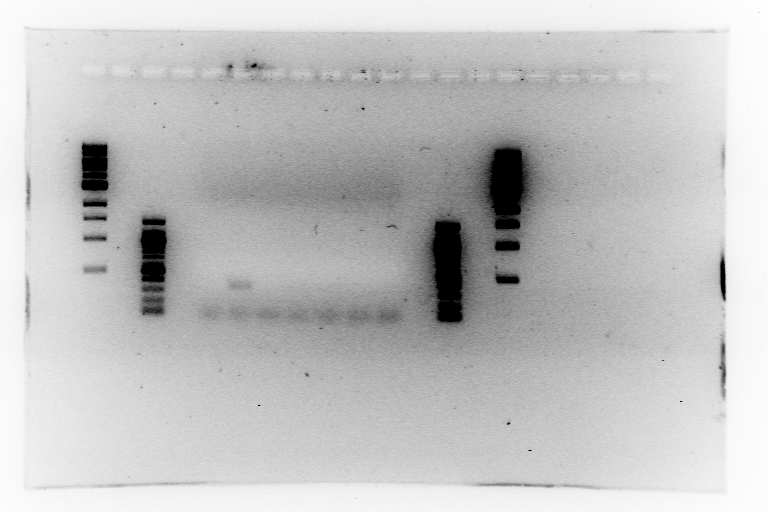
\includegraphics[width=\textwidth]{graphics/pic/20180210_EMP_OneTaq_MasterPure_vs_AllPrep.png}
        \caption{With EMP primers}
        \label{sfig:20180210_EMP_OneTaq_MasterPure_vs_AllPrep}
    \end{subfigure}
    ~ 
    \begin{subfigure}[b]{0.3\textwidth}
        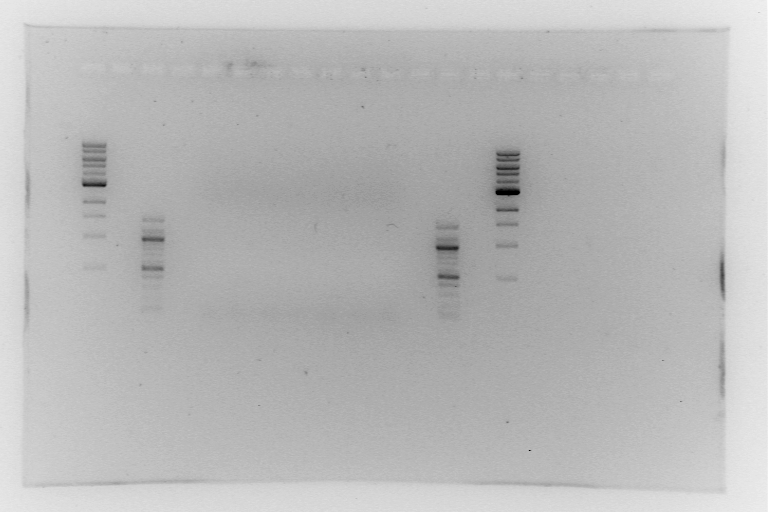
\includegraphics[width=\textwidth]{graphics/pic/20180210_ARCH_OneTaq_MasterPure_vs_AllPrep.png}
        \caption{With ARCH primers}
        \label{sfig:20180210_ARCH_OneTaq_MasterPure_vs_AllPrep}
    \end{subfigure}
    ~ 
    \begin{subfigure}[b]{0.3\textwidth}
        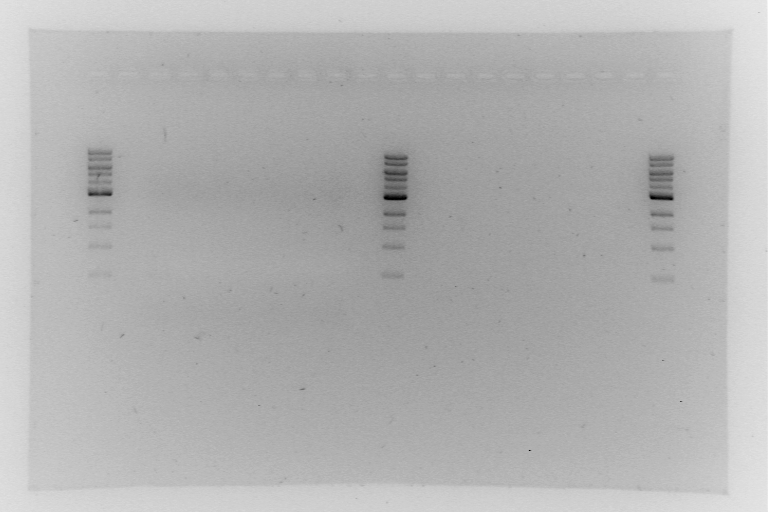
\includegraphics[width=\textwidth]{graphics/pic/20180210_EUK1_OneTaq_MasterPure_vs_AllPrep.png}
        \caption{With EUK1 primers}
        \label{sfig:20180210_EUK1_OneTaq_MasterPure_vs_AllPrep}
    \end{subfigure}
\end{figure}

In figure \ref{sfig:20180210_EMP_OneTaq_MasterPure_vs_AllPrep}, only the positive control for bacteria amplified. But the archaea positive control did not work. For the other primers, the reactions did not work at all. Maybe I put too little DNA template in the mix which is why it does not amplified. So I should try again with less than 5~\uL of DNA templates but more than 1~\uL.
